\documentclass[a4paper, oneside, british]{memoir}
\usepackage[datesep=/]{datetime2}

\usepackage{hyperref}
\PassOptionsToPackage{hidelinks}{hyperref}
\hypersetup{pdfborder=0 0 0}

\usepackage[backend=biber, style=ieee]{biblatex}
\addbibresource{main.bib}

\usepackage{fontspec}
\setmainfont{Arial}
\newfontfamily{\arial}{Arial}
\newfontfamily{\fauna}{FAUNA}[Path = fonts/, Extension = .ttf, UprightFont = *-THIN]

\usepackage{cascadia-code}

\usepackage{lastpage}
\usepackage{pgfplots}
\usepackage{geometry}
\usepackage{bookmark}
\usepackage{hyperref}
\usepackage{enumitem}
\usepackage{calc}
\usepackage{longtable}
\usepackage{graphicx}
\usepackage{wrapfig}
\usepackage{listings}
\usepackage{amsmath}
\usepackage{bytefield}
\usepackage{pdfpages}
\usepackage{tikz}
\usepackage{tabularx}
\usepackage{amsmath}
\usepackage{array}
\usepackage{titlesec}
\usepackage{varwidth}
\usepackage{bytefield}
\usepackage{siunitx}
\usepackage{hyperref}
\usepackage{graphicx}
\usepackage{tcolorbox}
\usepackage{bm}
\usepackage{svg}
\usepackage{lipsum}
\usepackage{fontawesome}

\pagestyle{empty}

% ======================================================================================
%                                         MISC
% ======================================================================================

\setlist[itemize]{noitemsep}
\setlist[itemize, 1]{itemsep=0.5em,align=parleft,left=0pt..1.5em, label={\Large\textbullet}}

% Set up SI units
\sisetup{group-separator = {,}} % Separate groups with comma (i.e. 1,000,000)
\DeclareSIUnit{\feet}{ft}       % Add custom non SI unit for feet 

% Date style to display only the year
\DTMnewdatestyle{yearonly}{%
    \renewcommand{\DTMdisplaydate}[4]{\number##1}
    \renewcommand{\DTMDisplaydate}{\DTMdisplaydate}
}

% Define \setdocname to store the document name
\newcommand{\setdocname}[1]{\def\docname{#1}}
\newcommand{\docname}{}

% Define \setsysname to store the system name
\newcommand{\setsysname}[1]{\def\sysname{#1}}
\newcommand{\sysname}{}

% Define \setorglabel to store the organisation label
\newcommand{\setorglabel}[1]{\def\orglabel{#1}}
\newcommand{\orglabel}{}

% ======================================================================================
%                                    HEADER/FOOTER
% ======================================================================================

% Remove chapter/section number from rightmark
\makepsmarks{ruled}{%
 \nouppercaseheads
 \createmark{chapter}{right}{nonumber}{}{}
 \createmark{section}{right}{nonumber}{}{}
}

% Make header/footer rules full headwidth
\makerunningwidth{ruled}{\headwidth}

% Header/footer rules
\makeheadrule{ruled}{\headwidth}{2\normalrulethickness}
\makefootrule{ruled}{\headwidth}{2\normalrulethickness}{-0.20in}

% Change header/footer text & logo (use odds for single side)
\makeoddhead{ruled}{\textbf{\docname}}{}{\textbf{\rightmark}}
\makeoddfoot{ruled}{\small \thepage/\pageref{LastPage}}{\small \orglabel}{\includesvg[width=100pt]{./img/logo.svg}}

% ======================================================================================
%                                      SECTIONING
% ======================================================================================

% Set margins
%\setlrmarginsandblock{1in}{1in}{*} 
\setlrmarginsandblock{1.25in}{1.25in}{*} 
\setulmarginsandblock{1.25in}{1.25in}{*} 
\checkandfixthelayout%

% Define length to dedent text from margin to header width
\newlength{\margindedent}
\setlength{\margindedent}{0.5\textwidth-0.5\headwidth}

% Section title format 
\titleformat*{\section}{\huge\bfseries}
\titleformat*{\subsection}{\Large\bfseries}
\titleformat*{\subsubsection}{\large\bfseries}

% Section number format
\renewcommand{\thesection}{\arabic{section}}
\renewcommand{\thefigure}{\arabic{section}.\arabic{figure}}
\renewcommand{\thetable}{\arabic{table}}
\renewcommand{\abstractname}{Introduction}

% Label figures within sections
\numberwithin{figure}{section}

% Numbering
\setsecnumformat{\csname the#1\endcsname\hspace{0.5in-\widthof{\csname the#1\endcsname}}}
\setsecnumdepth{paragraph}

% Indentation
\setsecindent{1\margindedent}
\setsubsecindent{1\margindedent}
\setsubsubsecindent{1\margindedent}

\setlength{\absleftindent}{0em}
\setlength{\absrightindent}{0em}

\renewcommand{\baselinestretch}{1.125} % Scale baselineskip length
\setlength{\parskip}{0.5em}            % Adjust paragraph spacing

% ======================================================================================
%                                      LISTINGS
% ======================================================================================

\lstset{language=C++,
        basicstyle=\ttfamily,
        keywordstyle=\color{blue}\ttfamily,
        stringstyle=\color{red}\ttfamily,
        commentstyle=\color{lightgreen}\ttfamily,
        morecomment=[l][\color{magenta}]{\#},
        numbers = left,
        breaklines = true
}

% Suppress numbering
\let\origthelstnumber\thelstnumber
\makeatletter
\newcommand*\Suppressnumber{%
  \lst@AddToHook{OnNewLine}{%
    \let\thelstnumber\relax%
  }%
}

% Restore numbering
\newcommand*\Reactivatenumber{%
  \lst@AddToHook{OnNewLine}{%
   \let\thelstnumber\origthelstnumber%
  }%
}
\makeatother

% ======================================================================================
%                                          TIKZ
% ======================================================================================

\newenvironment{xcenter}
 {\par\setbox0=\hbox\bgroup\ignorespaces}
 {\unskip\egroup\noindent\makebox[\textwidth]{\box0}\par}

\usetikzlibrary{positioning,fit,calc,chains,matrix,arrows.meta,shapes.geometric,arrows,backgrounds}

\pgfdeclarelayer{subbackground}
\pgfdeclarelayer{background}
\pgfdeclarelayer{foreground}
\pgfsetlayers{subbackground,background,main,foreground}

\tikzstyle{square} = [regular polygon, regular polygon sides=4, draw=black, inner sep=0cm, align=center]

% Flowchart shapes
\tikzstyle{start} = [rectangle, rounded corners, minimum width=3cm, minimum height=1cm, text centered, draw=black, fill=green!30]
\tikzstyle{stop} = [rectangle, rounded corners, minimum width=3cm, minimum height=1cm, text centered, draw=black, fill=red!50]
\tikzstyle{process} = [rectangle, minimum width=3cm, minimum height=1cm, text centered, draw=black, fill=orange!80, text=white]
\tikzstyle{decision} = [diamond, minimum width=3cm, minimum height=3cm, text centered, draw=black, fill=blue!50, text=white]
\tikzstyle{arrow} = [thick,->,>=stealth, draw=blue, text=blue]

\tikzstyle{board} = [
  rectangle, dashed, very thick, rounded corners, 
  minimum width=1cm, minimum height=1cm, inner sep=0.25cm,
  draw=gray
]
\tikzstyle{group} = [
  rectangle, very thick, rounded corners, 
  minimum width=1cm, minimum height=1cm, inner sep=0.25cm,
  draw=gray, fill=gray!25
]
\tikzstyle{second_group} = [
  rectangle, dashed, very thick, rounded corners, 
  minimum width=1cm, minimum height=1cm, inner sep=0.25cm,
  draw=gray, fill=white!5
]

\tikzstyle{element} = [rectangle, rounded corners, text centered, draw=black, minimum width=2cm, minimum height=1cm, fill=white]

\tikzstyle{register} = [rectangle, rounded corners, text centered, draw=black, minimum width=3cm, minimum height=1cm, fill=white]
\tikzstyle{inout} = [trapezium, draw=black, minimum width=2cm, fill=white]

% Colours
\definecolor{bittersweet}{rgb}{1.0, 0.44, 0.37}
\definecolor{aquamarine}{rgb}{0.5, 1.0, 0.83}
\definecolor{lavender}{rgb}{0.9, 0.9, 0.98}
\definecolor{whitesmoke}{rgb}{0.96, 0.96, 0.96}
\definecolor{pastelred}{RGB}{242,220,218}
\definecolor{pastelgreen}{RGB}{216,227,192}
\definecolor{pastelyellow}{RGB}{254,242,205}
\definecolor{lightgreen}{RGB}{102,153,0}    %#669900

% ======================================================================================
%                                   TABLE OF CONTENTS
% ======================================================================================
\makeatletter
\renewcommand{\@pnumwidth}{-3em}
\renewcommand{\@tocrmarg}{-4em}
\makeatother
 
% Lengths
% -------------------------------------------------------------------------
% Defines the width of a section number in the ToC
\newlength{\tocsecnumwidth}
\setlength\tocsecnumwidth{10ex}

% Defines the standard width of a subsection number in the ToC
\newlength{\tocsubsecnumwidth}
\setlength\tocsubsecnumwidth{7ex}

% This is a useful shorthand for defining the indents of entry
% titles as offsets from the top level title indent
\def\tocentrytitleindent#1{\margindedent + \tocsecnumwidth + #1}
% -------------------------------------------------------------------------

\renewcommand*{\tocheadstart}{\vspace*{-1em}}
\renewcommand*{\aftertoctitle}{\vspace*{-0.5em}}
\setcounter{secnumdepth}{3}
\setcounter{tocdepth}{3}

% Make section trailing dots bold in ToC
\renewcommand{\cftsectionleader}{\bfseries\cftdotfill{\cftdotsep}}

% ToC title format
\renewcommand\contentsname{\textbf{Contents}}         % Make title bold
\renewcommand{\printtoctitle}[1]{                     % Head align ToC title
    \hspace{\margindedent}\huge #1\vspace{1em}
} 

% ToC entry format
\renewcommand{\cftsectionfont}{\Large\bfseries}       % Make section titles bold and Large
\renewcommand{\cftsubsectionfont}{\large}             % Make subsection titles large
\renewcommand{\cftsubsubsectionfont}{\large}          % Make subsubsection titles large

% ToC before entry skip
\newlength{\tocentryspace}
\setlength\tocentryspace{0.5em}                         % Standard skip 
\setlength\cftbeforesectionskip{3\tocentryspace}       % Extra space for sections
\setlength\cftbeforesubsectionskip{\tocentryspace}     % Standard skip for subsections
\setlength\cftbeforesubsubsectionskip{\tocentryspace}  % Standard skip for subsubsections

% ToC entry num width
\setlength\cftsectionnumwidth{\tocsecnumwidth}
\setlength\cftsubsectionnumwidth{\tocsubsecnumwidth}
\setlength\cftsubsubsectionnumwidth{\tocsubsecnumwidth + 1ex}

% ToC entry title indentation
\setlength\cftsectionindent{\margindedent}
\setlength\cftsubsectionindent{\tocentrytitleindent{0pt}}
\setlength\cftsubsubsectionindent{\tocentrytitleindent{\cftsubsectionnumwidth}}

\setlength\cftbeforechapterskip{0pt}

% List of equations
\newcommand{\listequationsname}{List of Equations}
\newlistof{listofequations}{equ}{\listequationsname}
\newcommand{\myequation}[1]{%
	\addcontentsline{equ}{equation}{\protect\numberline{\theequation}#1}\par
}
\makeatletter
\let\l@equation\l@figure
\makeatother

% Add lists
\addtocontents{lot}{\vskip -1.2cm} % List of tables
\addtocontents{equ}{\vskip -1.2cm} % List of equations

% ======================================================================================
% =                                                                                    = 
% =                                 BIBLIOGRAPHY                                       =
% =                                                                                    =
% ======================================================================================

% Bibliography heading
\defbibheading{references}[References]{%
 \clearpage\section{#1}
}

% ======================================================================================
%                                      TITLE FORMAT
% ======================================================================================

% CHANGE TITLE FORMATTING
\newcommand*{\titleAM}[2]%
{\begingroup
  \centering
  {\Huge #1 Documentation}\par\vspace{1em}
  {\huge #2}\par\vspace{1em}
  {\small {\DTMsetdatestyle{yearonly}\today} \orglabel}\par
  \endgroup}

% CHANGE DOCUMENT INFORMATION
\newcommand*{\documentInfo}[2]%
{\begingroup
  \centering
  \begin{table}[h]
  \centering
  \begin{tabularx}{0.5\textwidth}{@{}X@{}}
    Version      \dotfill #1     \\
    Last Updated \dotfill \today \\
    Date Created \dotfill #2     
  \end{tabularx}
  \end{table}
  \endgroup}

% ======================================================================================
% =                                                                                    = 
% =                                 DOCUMENT BODY                                      =
% =                                                                                    =
% ======================================================================================

% !!!!!!!!!!!!!!!!!!!!!!!!!!!! %
% DELETE THIS IN YOUR DOCUMENT %
% !!!!!!!!!!!!!!!!!!!!!!!!!!!! %
\AddToHook{shipout/foreground}{
  \begin{tikzpicture}[remember picture,overlay]
    \node[black,rotate=30,scale=15,opacity=0.15] at (current page.center) {EXAMPLE}; 
  \end{tikzpicture}
}

\begin{document}

  % !!!! THESE ARE DOCUMENT SPECIFIC !!!!
  % !!! CHANGE THESE IN YOUR DOCUMENT !!!
  \setorglabel{Example Organisation} 
  \setsysname{Example System}
  \setdocname{Document Title}

  % COVER PAGE
  % ----------------------------------------------------------------------------------

  \vspace*{-1in}
  \noindent\makebox[\textwidth]{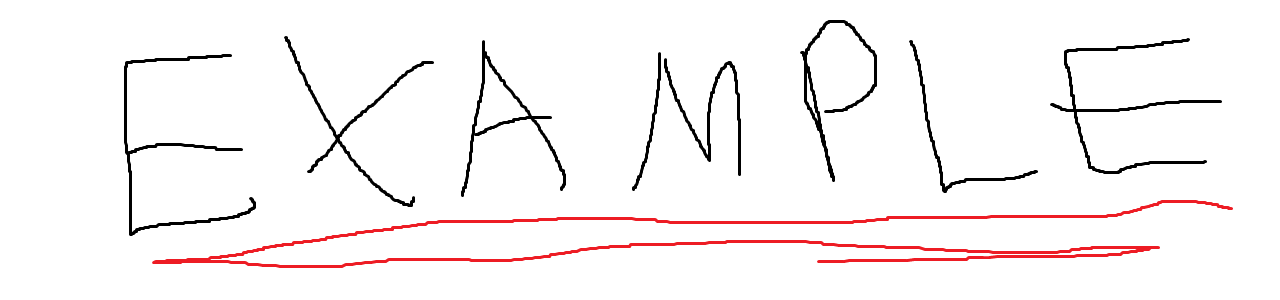
\includegraphics[width=\paperwidth]{./img/banner.png}}

  % COVER PAGE INTRODUCTION
  % !!! CHANGE THIS IN YOUR DOCUMENT !!!
  \section*{\hspace{-\margindedent}Introduction}
  \noindent\lipsum[1][1-5]\\[0.5em]
  \noindent\lipsum[1][5-8]\\[0.5em]
  \noindent\lipsum[1][8-13]
  
  % COVER PAGE RELATED DOCUMENTS
  % !!! CHANGE THIS IN YOUR DOCUMENT !!!
  \section*{\hspace{-\margindedent}Related Documents}
  Available from [repository name] (\url{https://www.github.com/repo-name}):
  \vspace{-0.5em}
  \begin{itemize}
    \item Technical reference
    \item Hardware manual
    \item Design review
    \item Test criteria and evaluation
    \item The Holy Bible
  \end{itemize}
  
  % COVER PAGE ACKNOWLEDGEMENTS
  % !!! CHANGE THIS IN YOUR DOCUMENT !!!
  \section*{\hspace{-\margindedent}Acknowledgements}
  \noindent\lipsum[1][1-8]\\[0.5em]
  \noindent\lipsum[1][8-14]

  \clearpage

  % ----------------------------------------------------------------------------------

  % DOCUMENT INFO
  % ----------------------------------------------------------------------------------
  
  \vspace*{\fill}
  
  % TITLE
  \titleAM{\sysname}{\docname}
  \documentInfo{1.0}{\DTMdate{2025-03-11}}

  % CHANGELOG
  \begin{table}[h]
  \centering
  \begin{tabularx}{0.6\textwidth}{lll}
  Date & Changes Made & Made By \\
  \midrule
  \DTMdisplaydate{2024}{12}{4}{-1} & Create initial document & Matthew Ricci\\
  \midrule
  \end{tabularx}
  \end{table}  

  \vspace*{\fill}
  
  %     This is for adding any document content unrelated to title/contents pages 
  % ⌄⌄⌄ to place before the table of contents itself
  \clearpage
  \input{precontent}
  \clearpage
  
  % ----------------------------------------------------------------------------------

  % CONTENTS
  \tableofcontents*
  \thispagestyle{ruled}

  % MAIN DOCUMENT
  \clearpage
  \markboth{}{}
  \pagestyle{ruled}

\begin{abstract}
Document descriptions at $\qty{10 000}{\feet}$~\cite{example} and $\qty{30 000}{\feet}$~\cite{example,example2,example3}.
\end{abstract}

\section{Section}

\subsection{Subsection}
\subsubsection{Subsubsection}
\subsubsection{Subsubsection}
\subsubsection{Subsubsection}
\subsubsection{Subsubsection}

\subsection{Subsection}
\subsection{Subsection}
\subsection{Subsection}
\subsection{Subsection}

\clearpage

\section{Firmware Architecture}
\begin{figure}[h]
    \centering
    \begin{tikzpicture}
        % Core ------------------------------------------------------------------------------------
        \node[element, minimum width=8cm, fill=pastelyellow!50](core){Australis Core};
        \node[element, minimum width=3cm, above=5mm of core.north, xshift=-2.15cm, fill=pastelgreen!50](core_state){State};
        \node[element, minimum width=3cm, above=5mm of core.north, xshift=2.15cm, fill=pastelgreen!50](core_devices){Devices};
        % Core group
        \begin{pgfonlayer}{background}
            \node[second_group, fit={(core_state) (core_devices)}](group_rectangle)(inner_main_group){};
        \end{pgfonlayer}
        \begin{pgfonlayer}{subbackground}
            \node[group, fit={(inner_main_group) (core)}, minimum width=4cm](group_rectangle)(main_group){};
        \end{pgfonlayer}
        % Extra ------------------------------------------------------------------------------------
        \node[element, minimum width=3cm, above=12.5mm of core_state.north, fill=pastelyellow!50](extra){Australis Extra};
        \node[element, minimum width=3cm, above=12.5mm of core_devices.north](target){Target\textsuperscript{1}};
        % Extra group
        \begin{pgfonlayer}{background}
            \node[group, fit={(extra) (target)}, minimum width=8.5cm](group_rectangle)(extra_group){};
        \end{pgfonlayer}
        % Legend -----------------------------------------------------------------------------------
        \node[square, minimum width=4mm, anchor=north west, above=5mm of extra_group.north west, xshift=7mm, draw=black, fill=pastelyellow, label={right:Australis Firmware}](legend_firmware){};
        \node[square, minimum width=4mm, right=of legend_firmware, xshift=3cm, draw=black, fill=pastelgreen, label={right:Australis Interface}](legend_interface){};
        % Subscript --------------------------------------------------------------------------------
        \node[anchor=west](sub) at ([yshift=-7mm, xshift=-2mm]core.south west) {\textsuperscript{1} Target component is implementation specific.};
        \useasboundingbox (current bounding box);
        % Labels -----------------------------------------------------------------------------------
        \node[label, left=of main_group]{Australis Core layer};
        \node[label, left=of extra_group]{Australis Target layer};
        % Arrows -----------------------------------------------------------------------------------
        \draw[-Triangle,thick] (core_state.north) |- ([yshift=-5mm]target.south) -- (target.south);
        \draw[-Triangle,thick] (core_devices.north) |- ([yshift=-5mm]extra.south) -- (extra.south);
        \draw[Triangle-Triangle,thick] (extra.east) -- (target.west);
    \end{tikzpicture}
    \caption{Australis Firmware system architecture}
\end{figure}

\clearpage

\section{Memory and Bus Architecture}
\subsection{System Architecture}

In STM32F405xx/07xx and STM32F415xx/17xx, the main system consists of 32-bit 
multilayer AHB bus matrix that interconnects:
\begin{itemize}
    \item Eight masters:
    \begin{itemize}
        \item Cortex\textsuperscript{\textregistered}-M4 with FPU core I-bus, D-bus, and S-bus
        \item DMA1 memory bus
        \item DMA2 memory bus
        \item DMA2 peripheral bus
        \item Ethernet DMA bus
        \item USB OTG HS DMA bus
    \end{itemize}
    \item Seven slaves:
    \begin{itemize}
        \item Internal flash memory ICode bus
        \item Internal flash memory DCode bus
        \item Main internal SRAM1 (112 KB)
        \item Auxiliary internal SRAM2 (16 KB)
        \item AHB1 peripherals including AHB to APB bridges and APB peripherals
        \item AHB2 peripherals
        \item FSMC
    \end{itemize}
\end{itemize}

\noindent The bus matrix provides access from a master to a slave, enabling concurrent access and 
efficient operation even when several high-speed peripherals work simultaneously. 
The 64-Kbyte CCM (core coupled memory) data RAM is not part of the bus matrix and can be 
accessed only through the CPU. This architecture is shown in Figure 1.

\vfill{}
\begin{center}
EXAMPLE DOCUMENT \\ \small (totally not stolen from RM0090)
\end{center}
\vfill{}

  % REFERENCES
  \renewcommand*{\UrlFont}{\rmfamily}
  \printbibliography[heading=references]

  % APPENDIX
  \clearpage
  \sectionmark{Appendix}
\phantomsection
\section*{Appendix}
\addcontentsline{toc}{section}{\hspace{\tocsecnumwidth}Appendix}

\setsecnumformat{Appendix \csname the#1\endcsname:\ }
\renewcommand{\thesubsection}{\Alph{subsection}}
\renewcommand{\thefigure}{\Alph{subsection}.\arabic{figure}}

\subsection{Appendix Item}


\end{document}
